%\documentclass[twoside]{article}
%
%\usepackage[margin=4cm]{geometry}
%\usepackage{calligra}
%\usepackage[colorlinks, linkcolor=azulsema!60!black]{hyperref}
%\usepackage{wrapfig}
%\usepackage{multicol}
%\usepackage{subfigure}
%%
%\usepackage[font=footnotesize,labelfont=bf]{caption}
%%
%\usepackage{eurosym}
%\usepackage[latin1]{inputenc}
%\usepackage[T1]{fontenc}
%\usepackage[spanish]{babel}
%\usepackage{colortbl}
%\usepackage{float}
%
%
%\usepackage{tikz}
%\usetikzlibrary{babel,calc,intersections,through,backgrounds,shadings,fadings}
%
%\definecolor{azulsema}{cmyk}{0.83, 0.3, 0.18, 0.11}
%\definecolor{azulcielo}{cmyk}{0.69, 0.42, 0.11, 0.03}
%
%\begin{document}
%\shorthandoff{>}\shorthandoff{<} %Necesario para compatibilizar los paquetes [spanish]{babel} 
%

\section{Eleuterio Toro publica el libro autobiogr\'afico: Exiliado en Buckingham Palace}

\begin{center}\large
\textbf{M� Elena V\'azquez Cend\'on}\\
Universidade de Santiago de Compostela  \\
{\color{azulsema}\rule{.5\linewidth}{1pt}}
\end{center}


\begin{figure}[h]
\centering
%\vspace*{-.9em}
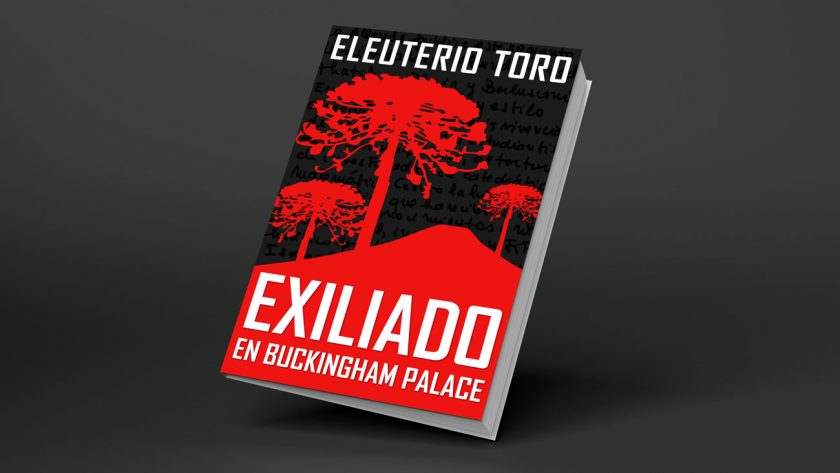
\includegraphics[width=0.8\textwidth]{exiliado-840x473.jpg}
\caption{Portada de \textbf{Exiliado en Buckingham Palace}.}
%\vspace*{-1.4em}
\end{figure}
Las personas que hemos tenido la fortuna de compartir Matem\'aticas con Eleuterio Francisco Toro sabemos que, adem\'as de ser un referente internacional en Resolventes de Riemann, es un ser humano admirable. Si adem\'as hemos podido departir con \'el en mesas con mantel, podemos dar fe de que ha sabido descentrar con \'exito muchas adversidades. 

El libro \url{https://eleuteriotoro.com/exiliado_buckingham_palace}, protagonista de la rese\~na, depende de variables espaciales y temporales que viven en el dominio de definici\'on de nuestro amigo y que explican inc\'ognitas, como su propio nombre, al que por ventura no renunci\'o. En palabras suyas: <<Recuento mis vivencias de ni\~no campesino, maestro, estudiante universitario, l\'ider estudiantil, prisionero, torturado, escapado, despatriado, exiliado, investigador matem\'atico y catedr\'atico>>. 

Sin perder el humor chileno, pr\'oximo a la retranca gallega, nuestro amigo destina rigor cient\'ifico de alto orden a la hora de reflexionar sobre <<educaci\'on, la matem\'atica en la escuela y en la vida; la investigaci\'on matem\'atica y sus aplicaciones en diversas \'areas del conocimiento humano, incluida la medicina>>.


Hace ya dos a\~nos invit\'e a Tito a participar en el {\it Consello da Cultura Galega} en las jornadas tituladas {\textit{Persoas refuxiadas ConCiencia. An\'alise da problem\'atica das persoas refuxiadas desde a Ciencia e como persoas xeradoras de co\~necemento}, el t\'itulo de su ponencia fue similar al del libro, cuya primera versi\'on compartiera conmigo. En este enlace pod\'eis escucharlo, presentado por uno de los personajes del libro, su hermano Gino, \url{http://consellodacultura.gal/persoa.php?id=8294}. 

Recomiendo el libro a todas las generaciones, para compartir que la Ciencia es permeable a las vivencias de las personas que la desarrollan y valorar que, adem\'as de dedicarle tiempo a las publicaciones con las que compartimos nuestras aportaciones, son de agradecer aquellas en las que compartimos las reflexiones vitales que tambi\'en producen Ciencia.

La memoria de este brillante acad\'emico conforma tambi\'en la Matem\'atica Aplicada por la que nuestra sociedad apuesta, al dar protagonismo a las personas que la desarrollan. Apelando a la memoria, comparto una foto del congreso en su honor que celebramos en Santiago de Compostela en 2011, con una importante presencia de miembros de la SEMA.

\vspace{2em}\par

\begin{figure}[h]
\centering
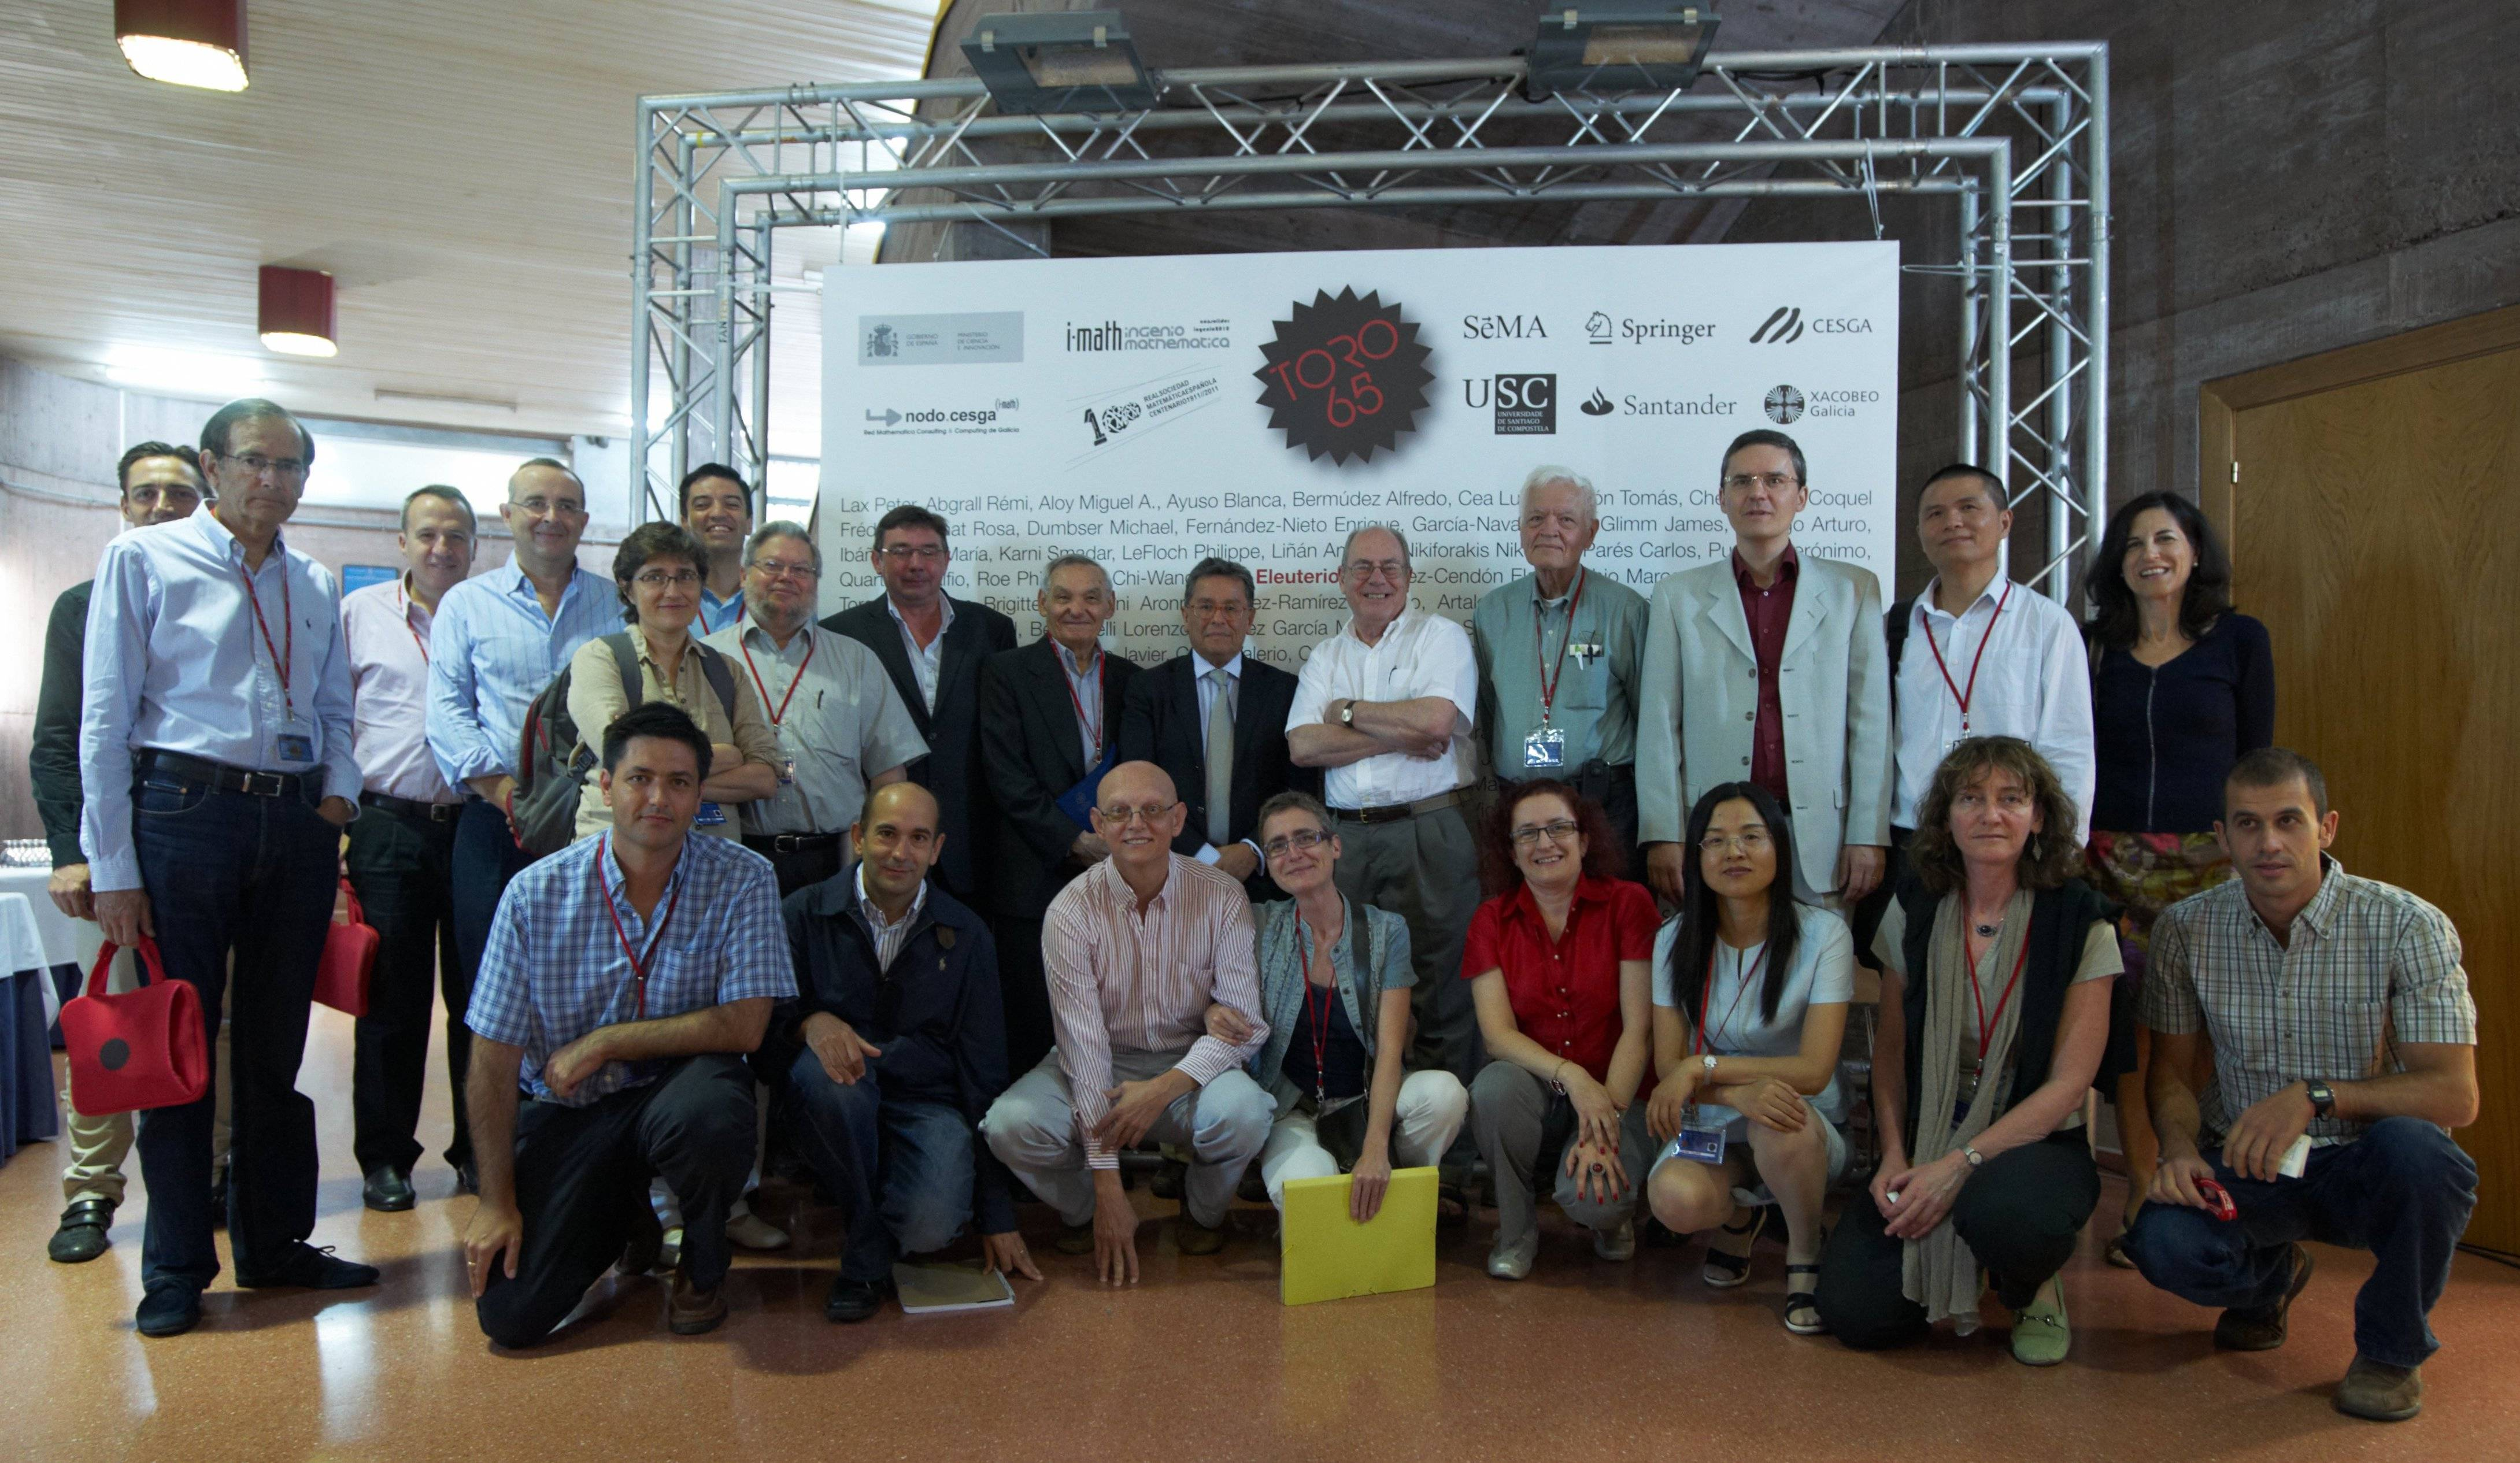
\includegraphics[width=\textwidth]{ToroySema.jpg}
\caption{E.~F. Toro y un buen n\'umero de miembros de SEMA en el Congreso en su honor en Santiago de Compostela en 2011.}
\end{figure}


\vspace{2em}\par

\begin{center}
\resizebox{.7\linewidth}{!}{\color{azulsema}\rule{.5\linewidth}{1pt}
{\large $\diamond$} {\huge $\diamond$} {\large $\diamond$} \rule{.5\linewidth}{1pt}}\\[.3ex]
\mbox{}
\end{center}

%
%\end{document}
%
%
%
%\end{document}
